\documentclass[20pt,A4]{article}
\usepackage{array}
\usepackage[centering, margin={1in, 0.8in}, includeheadfoot]{geometry}
\usepackage{graphicx}
\usepackage[table]{xcolor}
\usepackage{mathptmx}
\usepackage{anyfontsize}
\usepackage{t1enc}
\usepackage{background}
\usepackage[absolute,overlay]{textpos}

\setlength{\headheight}{0in} 
\setlength{\headsep}{0pt}
\setlength{\topmargin}{0pt}
\setlength{\footskip}{0pt}
\setlength{\marginparsep}{11pt}
\pagestyle{empty}

\backgroundsetup{contents=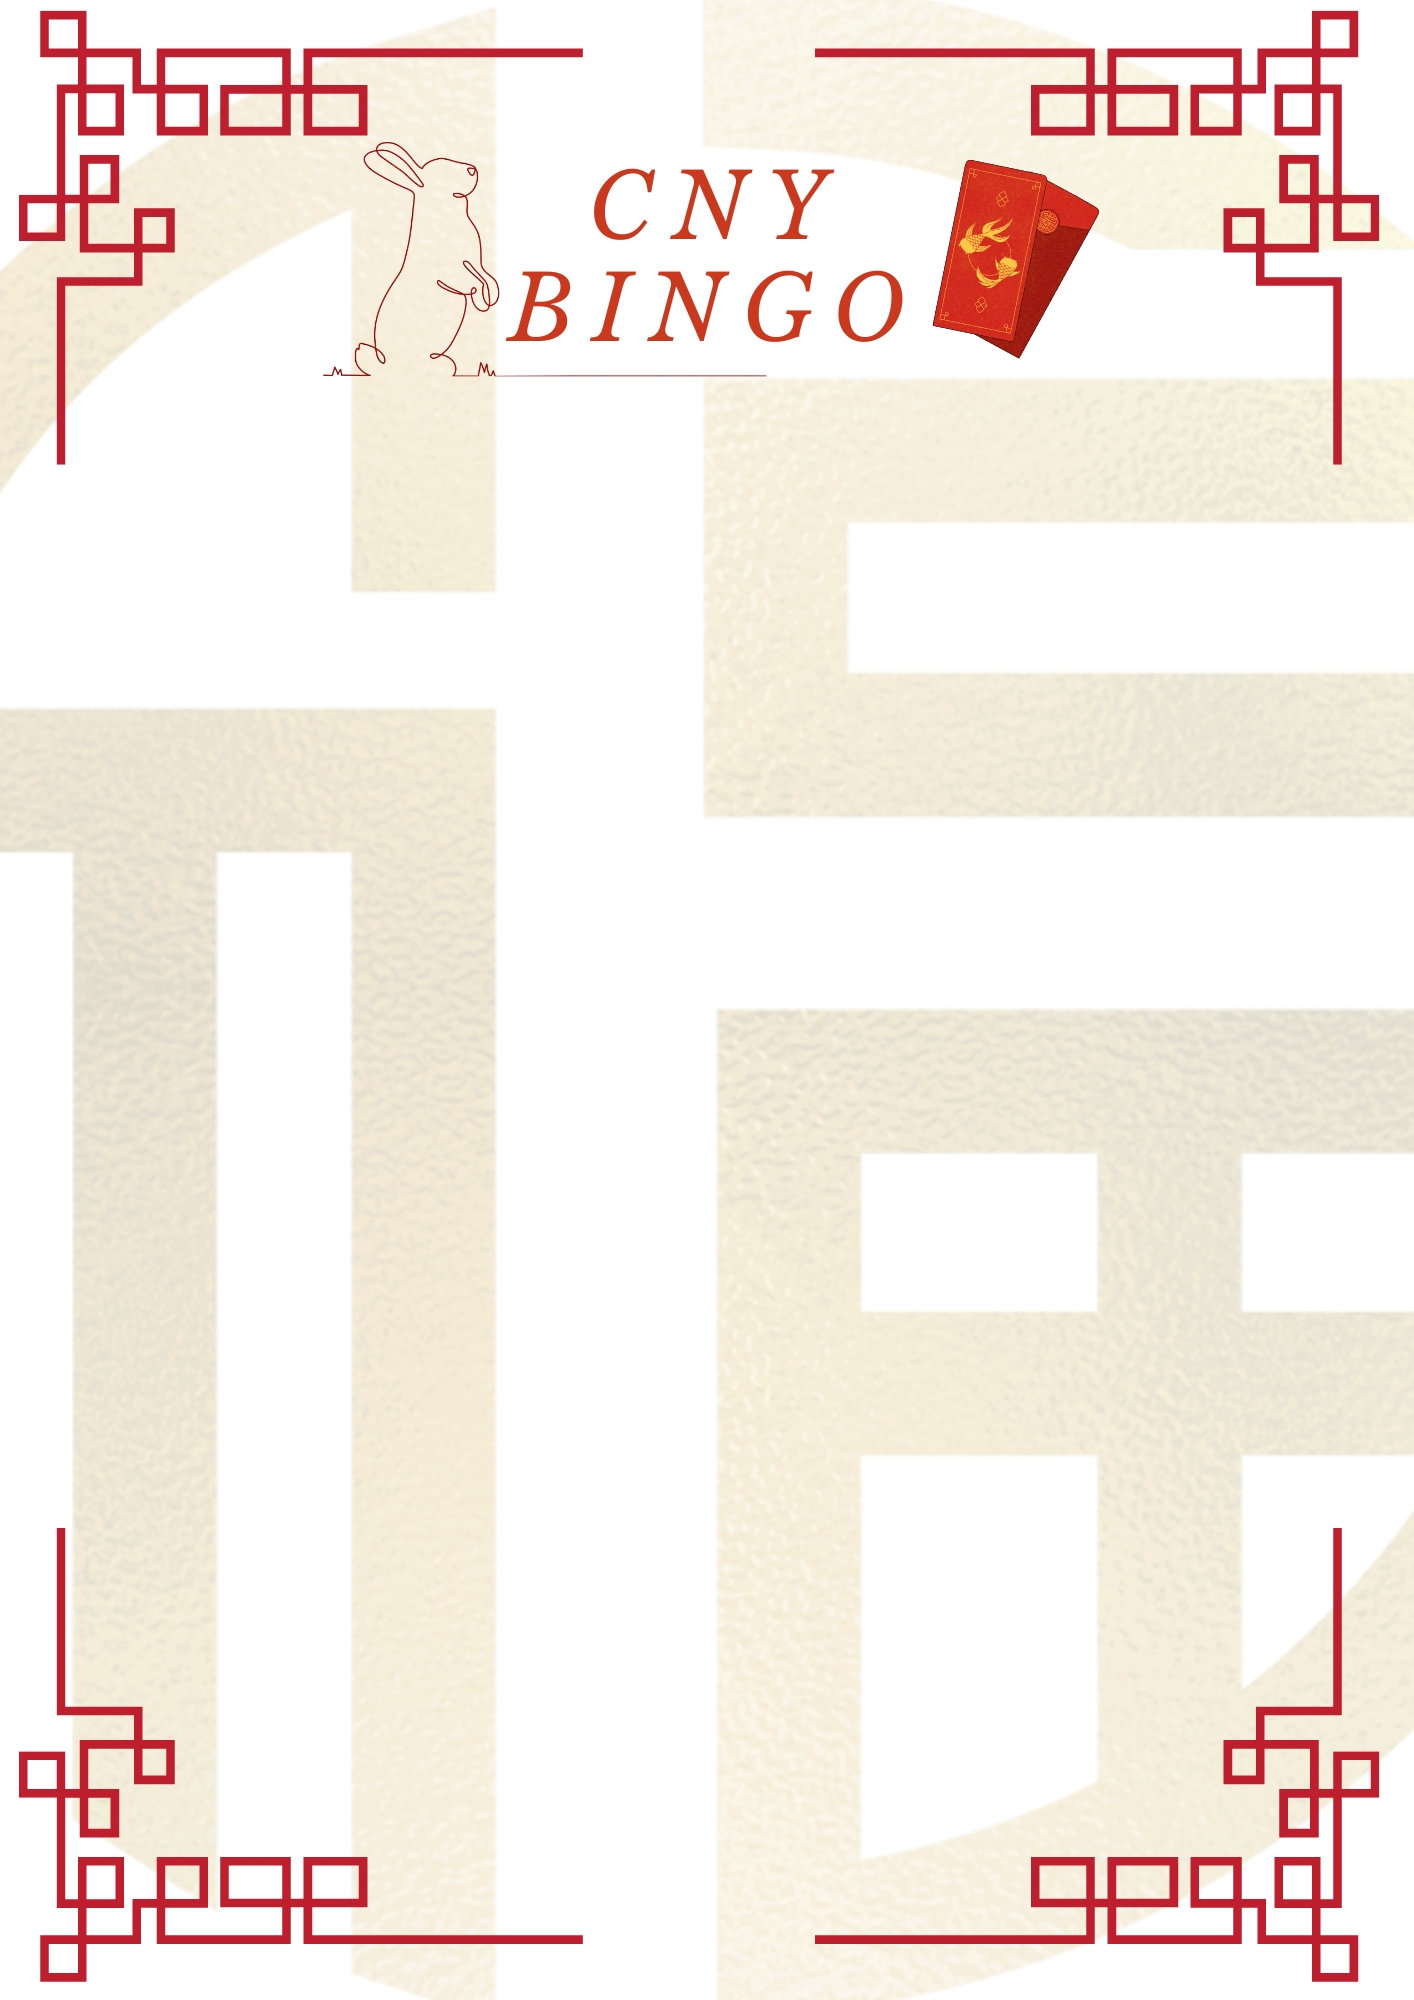
\includegraphics{cny.jpg}, hshift=0cm, vshift=1cm, angle=0, scale=0.38, opacity=0.85}
\newcolumntype{L}[1]{>{\raggedright\let\newline\\\arraybackslash\hspace{0pt}}m{#1}}
\newcolumntype{C}[1]{>{\centering\let\newline\\\arraybackslash\hspace{0pt}}m{#1}}
\newcolumntype{R}[1]{>{\raggedleft\let\newline\\\arraybackslash\hspace{0pt}}m{#1}}

\definecolor{darkred}{rgb}{1,0.35,0.25}

\begin{document}

\begin{textblock*}{3cm}(15.5cm,4cm)
   \Huge \textcolor{darkred}{01}
\end{textblock*}

\hphantom
\newline
\newline
\newline
\newline
\newline
\newline
\newline
\newline

\begin{center}
\large \bfseries
\begin{tabular}{| C{2.8cm}| C{2.8cm}| C{2.8cm}| C{2.8cm}| C{2.8cm}|} \hline  
Has the digit ‘8’ in their handphone number & Ate tang yuan during CNY &  Collected more than 8 Ang Paos this year  & Had food spilled on you during Lou Hei  & Has a birthday this month \\[2cm]
\hline 
 Has the digit ‘8’ in their house unit number & Put up CNY home deco & Had a relative questioned your life during CNY  & Set off firecrackers   & Played mahjong this CNY \\ [2cm]
\hline 
Received a negative fortune prediction for the new year & Ate more than 5 types of CNY snacks this year (name 5) & Born in this zodiac year  & Has been to China  & Wore traditional Chinese clothing during CNY \\ [2cm]
\hline 
 Wore matching clothes with family on CNY  & Can recite 2 CNY blessings (or more) & Had steamboat more than once this CNY  & Stayed up on CNY eve & Can recite 2 CNY blessings (or more) \\ [2cm]
\hline 
 Wore traditional Chinese clothing during CNY & Hung pineapple lanterns at home for CNY & Has the digit ‘8’ in their house unit number  & Watched “Our Times” on TV during house visiting  & Went to Chinatown during CNY \\ [2cm]
\hline 
 \end{tabular}
\end{center}

\centerline{\textcolor{darkred}{brought to you by the APHC Bonding Committee}}

\newpage

\begin{textblock*}{3cm}(15.5cm,4cm) 
   \Huge \textcolor{red}{02}
\end{textblock*}

\hphantom
\newline
\newline
\newline
\newline
\newline
\newline
\newline
\newline

\begin{center}
\large \bfseries
\begin{tabular}{| C{2.8cm}| C{2.8cm}| C{2.8cm}| C{2.8cm}| C{2.8cm}|} \hline  
Has the digit ‘8’ in their handphone number & Ate tang yuan during CNY &  Collected more than 8 Ang Paos this year  & Had food spilled on you during Lou Hei  & Has a birthday this month \\[2cm]
\hline 
 Has the digit ‘8’ in their house unit number & Put up CNY home deco & Had a relative questioned your life during CNY  & Set off firecrackers   & Played mahjong this CNY \\ [2cm]
\hline 
Received a negative fortune prediction for the new year & Ate more than 5 types of CNY snacks this year (name 5) & Born in this zodiac year  & Has been to China  & Wore traditional Chinese clothing during CNY \\ [2cm]
\hline 
 Wore matching clothes with family on CNY  & Can recite 2 CNY blessings (or more) & Had steamboat more than once this CNY  & Stayed up on CNY eve & Can recite 2 CNY blessings (or more) \\ [2cm]
\hline 
 Wore traditional Chinese clothing during CNY & Hung pineapple lanterns at home for CNY & Has the digit ‘8’ in their house unit number  & Watched “Our Times” on TV during house visiting  & Went to Chinatown during CNY \\ [2cm]
\hline 
 \end{tabular}
\end{center}

\end{document}